\section{The Need for Binary Analysis}
\label{vine:introduction}

% We would like to develop software security solutions that are widely
% applicable and offer strong guarantees. 

% We take a binary-centric approach to software security because binary
% code is everywhere, and binary code is faithful to what will actually
% be executed on hardware. Effective security-centric binary analysis
% techniques can potentially impact a wide audience, and provide strong
% guarantees as to what will actually be executed.

Binary code is everywhere. In most situations, users only have access
to code in binary (i.e., executable) form.  Most common, off-the-shelf
(COTS) software (e.g., Microsoft Windows, Adobe Acrobat, etc.) is only
available to end-users in binary form.  Malicious code (i.e., malware)
created by attackers is typically only available in binary form.  The
ubiquity of binary code ensures that security techniques which only
require access to the program binary are likely to be widely
applicable. Further, binary code analysis allows us to argue about the
security of the code that will run, not just the code that was
compiled.


A binary-centric approach to software security requires the ability to
perform program analysis on binary code. A program analysis (whether
it be static or dynamic) is an algorithm for determining the effects
of a set of statements in the programming language under
consideration.  Thus, a binary-centric approach requires 1) the
ability to analyze each instruction in a manner faithful to its
semantics, and 2) a method for encoding an algorithm over those
instructions.

However, there are two primary challenges to performing accurate and
faithful analysis on modern binary code. First, code analysis at the
binary level is different than source code because binary code lacks
many abstractions found in higher-level languages. Second, binary code
is significantly more complex than source code, which introduces new
engineering challenges for binary code analysis.  

% We have developed \emph{\bap}, a \underline{B}inary
% \underline{A}nalysis \underline{P}latform, which addresses these
% challenges. At the heart of \bap is a) a simplified, formally-specific
% intermediate language for assembly, and b) a set of core analysis that
% appropriate for binary code.

\paragraph{Binary Code Analysis is Different than Source Code Analysis.}
Binary code is different than source code. Thus, we must develop and
only use program analyses that are suitable for the unique
characteristics of binary code.  In particular, binary code lacks
abstractions that are often fundamental to source code and source code
analysis, such as:
\begin{itemize}
\item {\bf Functions.} The function abstraction does not exist at the
  binary level.  Instead, control flow in a binary program is
  performed by jumps. For example, the x86 instruction {\tt call x} is
  just syntactic sugar (i.e., shorthand) for storing the number in the
  instruction pointer register {\tt eip} at the address named by the
  register {\tt esp}, decrementing {\tt esp} by the architecture word
  size, and then loading the {\tt eip} with number {\tt x}. Indeed, it
  is perfectly valid in assembly, and sometimes happens in practice,
  that one may call into the middle of a ``function'', or have a
  single ``function'' separated into non-contiguous pieces. The lack
  of a function abstraction poses significant scalability challenges
  to binary analysis.

\item {\bf Memory vs. Buffers.} Binary code does not have buffers, it
  has \emph{memory}.  While the OS may determine a particular memory
  page is not valid, memory does not have the traditional semantics of
  a user-specified type and size. One implication of the difference
  between buffers and memory is that in binary code there is no such
  thing as a buffer overflow. While we may say a particular store
  violates a higher-level semantics given by the source code, such
  facts are inferences with respect to the higher-level semantics, not
  part of the binary code itself. The lack of buffers means we have to
  conservatively reason about the entire memory space (unless proven
  otherwise) at each operation.

\item {\bf No Types.} New types cannot be created or used since there
  is no such thing as a type constructor in binary code. The only
  types available are those provided by the hardware: registers and
  memory.  Even register types are not necessarily a good choice,
  since it is common to store values from one register type (e.g.,
  32-bit register) and read them as another (e.g., 8-bit
  register). The lack of types means we cannot use type-based
  analysis, which is often instrumental in scaling traditional
  analyses.

\end{itemize}


\paragraph{Binary Code is Complex.}

\begin{figure}
\begin{minipage}{.4\linewidth}
\begin{code}
// instr dst,src
1. add eax, ebx
2. shl eax, edx
3. jo target
4. ....
...
target: ...
\end{code}
\end{minipage}
\begin{minipage}[c]{.5\linewidth}
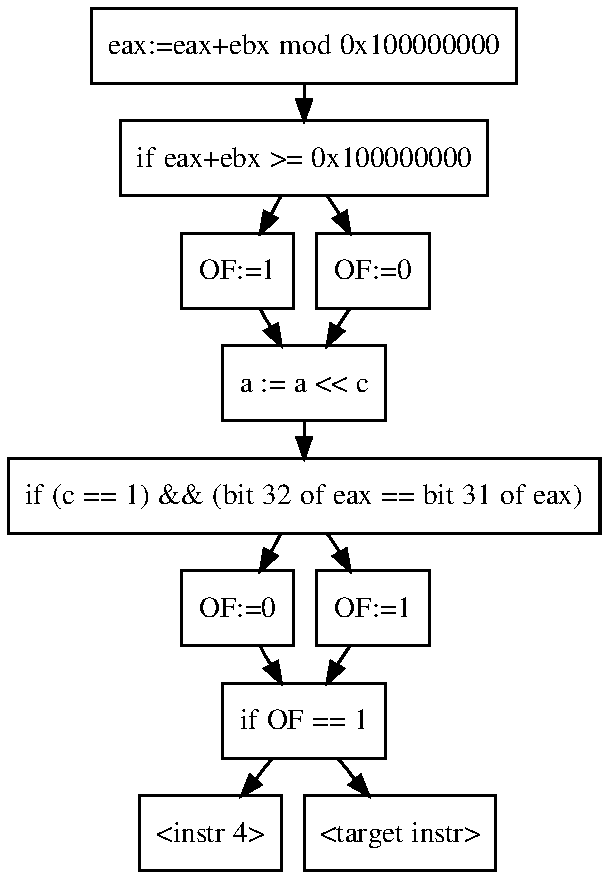
\includegraphics[scale=.5]{fig/add-shl}
\end{minipage}
\caption{A three instruction x86 program, and its corresponding
  control flow graph.  Note the logic for deciding when the jump on
  overflow instruction (statement 3) is taken, when is often omitted
  by other binary analysis platforms. }
\label{vine:shl-add}
\end{figure}

One approach is to disassemble binary code into a sequence of assembly
instructions, and then perform program analysis directly over the
assembly instructions.  This type of assembly-specific approach is
\naive because each analysis would have to individually understand the
semantics of the assembly, which is difficult.

For example, consider the basic program analysis problem of
determining when the conditional jump is taken on line 3 of
Figure~\ref{vine:shl-add}. In this example, all operands are 32-bit
registers, and all arithmetic is therefore performed mod
$2^{32}$. Instruction 1 computes the sum {\tt eax := eax+ebx} (mod
$2^{32}$).  Instruction 2 computes {\tt eax = eax $\ll$ edx}.  Both
instructions may set the overflow status register {\tt OF}. The {\tt
  add} instruction will set the {\tt OF} flag if {\tt eax + ebx $\geq$
  $2^{32}$}.  The {\tt shl} instruction will set the {\tt OF} flag if
{\tt edx} is 1 \emph{and} the top two bits of {\tt eax} are not equal
on line 2. The instruction on line 3 tests to see if {\tt OF} is set,
and if so, jumps to {\tt target}, else executes the next sequential
instruction. 

In order to determine when the jump on line 3 is taken, an analysis
must reconstruct all side-effects of {\tt add} and {\tt shl}.  The
proper control flow diagram is shown in Figure~\ref{vine:shl-add}.  As
demonstrated by this three line program, even though a program may
look simple, determining the effects may be complicated. An
assembly-specific approach would require each analysis to reason about
such complex semantics.


Worse, many architectures allow instruction prefixes, which can
further complicate the semantics. For example, in x86 a {\tt rep}
prefix essentially turns an instruction into a single instruction
loop, e.g., {\tt rep $i$ $s$,$d$} will repeatedly execute operation
$i$ on arguments $s$ and $d$.  The exact semantics (per
Intel~\cite{intel:x86}) of {\tt rep} are shown in
Figure~\ref{vine:rep}. An assembly-specific approach would have to
consider this complicated logic for any instruction that may carry the
{\tt rep} prefix. If analyses are written directly on assembly, each
analysis would duplicate this logic.


\begin{figure}
\begin{footnotesize}
\begin{code}
  IF AddressSize = 16 
  THEN 
     Use CX for CountReg; 
  ELSE IF AddressSize = 64 and REX.W used 
     THEN Use RCX for CountReg; FI; 
  ELSE 
     Use ECX for CountReg; 
  FI; 
  WHILE CountReg $\neq$ 0 
  DO 
      Service pending interrupts (if any); 
      Execute associated string instruction ($x$);  
      CountReg $\leftarrow$ (CountReg – 1); 
      IF CountReg = 0 
      THEN exit WHILE loop; FI; 
      IF (Repeat prefix is REPZ or REPE) and (ZF = 0) 
         or (Repeat prefix is REPNZ or REPNE) and (ZF = 1) 
      THEN exit WHILE loop; FI; 
  OD; 
\end{code}
\end{footnotesize}
\caption{The semantics of the {\tt rep} instruction according to
  Intel~\cite{intel:x86}. Modern architectures often have hundreds of
  instructions that have complex semantics like {\tt rep}.}
\label{vine:rep}
\end{figure}

If there were only a few instructions, perhaps the complexity would
not be too onerous.  Modern architectures, however, typically have
hundreds of instructions. x86, for example, has well over 300
instructions (which are documented in over 11 lbs of
manuals~\cite{intel:x86}).

% This is very outdated now.
% Overall, an assembly specific approach is unattractive because writing
% analyses over modern instruction sets tends to be tedious and
% error-prone. For example, the current version of
% DynInst~\cite{dyninst} (version 5.2) and Phoenix~\cite{phoenix} (April
% 2008 SDK Build), two popular architectures for binary analysis, will
% not create a correct control flow graph for the three line program.
% Verifying a program analysis is correct over a large and complicated
% instruction set seems even more difficult.
% Further, an
% assembly-specific approach is specific to a single architecture.  All
% analysis would have to be ported each time we want to consider a new
% architecture.  Thus, analysis could not take advantage of the common
% semantics across many different assemblies.


\section{Desired Properties}

We would like a platform for analyzing binary code that 1) supports
writing analyses in a concise and straight-forward fashion, 2)
provides abstractions for common semantics across all assemblies, and
3) is architecture independent when possible.

We want an architecture that supports writing analyses in a concise,
straight-forward fashion because that makes it easier to write
analyses that are correct.  We do not want an analysis to have to
tangle with complicated instruction semantics: that should be the
job of the architecture.  
%Simplifying analysis is challenging,
%however, because modern architectures are designed for computational
%efficiency, not ease of understanding.

We would also like to provide abstractions that are common to typical
program analyses. There are many recurring abstractions. One is to be
able to iterate over each instruction type. Another is to build a
control flow graph.  Yet another is finding data dependencies. We
would like to build a single platform so that a new program analysis
can easily reuse common abstractions.

Finally, we would like to be architecture independent.  Architecture
independence would allow us to easily re-target the entire platform to
a new architecture without changing the analyses.  The more
architectures we can handle, the more widely our techniques will be
applicable.



% modern instructions is likely at best to difficult to create,
% difficult to debug, and difficult to show correct.




% . One reason is an
% assembly-specific approach is specific to only the single assembly for
% the architecture under consideration. Second, writing program analysis
% over assembly directly is tedious and error-prone.  Modern
% architectures such as x86 typically have hundreds of instructions,
% each of which may have complex semantics.  As a result, a typical
% program analysis may have to consider hundreds of cases, and each case
% may be associated with extensive code to handle the complexity of a
% particular instruction.

%%% Local Variables: 
%%% mode: latex
%%% TeX-master: "../main"
%%% End: 
